\documentclass[a4paper,17pt]{extarticle}


    \usepackage[sfdefault, condensed]{roboto} % police d'écriture plus moderne
\usepackage[french]{babel} % francisation
\usepackage[parfill]{parskip} %suppression indentation

\usepackage{fancyhdr}
\usepackage{multicol}

% figure non flotantes
\usepackage{float}
\let\origfigure\figure
\let\endorigfigure\endfigure
\renewenvironment{figure}[1][2] {
    \expandafter\origfigure\expandafter[H]
} {
    \endorigfigure
}

% mois/année
\usepackage{datetime}
\newdateformat{monthyeardate}{%
  \monthname[\THEMONTH] \THEYEAR}

% couleurs perso
\usepackage[table]{xcolor}
\definecolor{deepblue}{rgb}{0.3,0.3,0.8}
\definecolor{darkblue}{rgb}{0,0,0.3}
\definecolor{deepred}{rgb}{0.6,0,0}
\definecolor{iremred}{RGB}{204,35,50}
\definecolor{deepgreen}{rgb}{0,0.6,0}
\definecolor{backcolor}{rgb}{0.98,0.95,0.95}
\definecolor{grisClair}{rgb}{0.95,0.95,0.95}
\definecolor{orangeamu}{RGB}{250,178,11}
\definecolor{noiramu}{RGB}{35,31,32}
\definecolor{bleuamu}{RGB}{20,118,198}
\definecolor{bleuamudark}{RGB}{15,90,150}
\definecolor{cyanamu}{RGB}{77,198,244}


\usepackage{/home/bouscadilla/Documents/Code/nbconvert/template/latex/pdf_solution/xeboiboites}
%
% exemple
\newbreakabletheorem[
    small box style={fill=deepblue!90,draw=deepblue!15, rounded corners,line width=1pt},%
    big box style={fill=deepblue!5,draw=deepblue!15,thick,rounded corners,line width=1pt},%
    headfont={\color{white}\bfseries}
        ]{exemple}{Exemple}{}%{counterCo}
%
% remarque
\newbreakabletheorem[
    small box style={draw=ansi-green-intense!100,line width=2pt,fill=ansi-green-intense!0,rounded corners,decoration=penciline, decorate},%
	big box style={color=ansi-green-intense!90,fill=ansi-green-intense!10,thick,decoration={penciline},decorate},
    broken edges={draw=ansi-green-intense!90,thick,fill=orange!20!black!5, decoration={random steps, segment length=.5cm,amplitude=1.3mm},decorate},%
    other edges={decoration=penciline,decorate,thick},%
    headfont={\color{ansi-green-intense}\large\scshape\bfseries}
    ]{remarque}{Remarque}{}%{counterCa}
%
% formule (sans titre)
\newboxedequation[%
    big box style={fill=cyanamu!10,draw=cyanamu!100,thick,decoration=penciline,decorate}]%
    {form}
%
% Réponse
\newbreakabletheorem[
    small box style={fill=bleuamu!100, draw=bleuamu!60, line width=1pt,rounded corners,decorate},%
    big box style={fill=bleuamu!10,draw=bleuamu!30,thick,rounded corners,decorate},
    headfont={\color{white}\large\scshape\bfseries}
        ]{reponse}{Correction}{}
%

%
% À retenir
%\newbreakabletheorem[
%    small box style={fill=deepred!100, draw=deepred!80, line width=1pt,rounded corners,decorate},%
%    big box style={fill=deepred!10,draw=deepred!50,thick,rounded corners,decorate},
%    headfont={\color{white}\large\scshape\bfseries}
%        ]{retenir}{À retenir}{}
%
\newboxedequation[%
    big box style={fill=deepred!10,draw=deepred!0,thick,decoration=penciline,decorate}]%
    {retenir}



% astuce
\newspanning[
    image=/home/bouscadilla/Documents/Code/nbconvert/template/latex/pdf_solution/fig-idee,headfont=\bfseries,
    spanning style={very thick,decoration=penciline,decorate}
    ]{astuce}{Astuce}{}
%
% activité
\newbreakabletheorem[
    small box style={draw=orangeamu!100,line width=2pt,fill=orangeamu!100,rounded corners,decoration=penciline, decorate},%
	big box style={color=orangeamu!100,fill=orangeamu!5,thick,decoration={penciline},decorate},
    broken edges={draw=orangeamu!100,thick,fill=orangeamu!100, decoration={random steps, segment length=.5cm,amplitude=1.3mm},decorate},%
    other edges={decoration=penciline,decorate,thick},%
    headfont={\color{white}\large\scshape\bfseries}
    ]{activite}{\adjustimage{height=1cm, valign=m}{/home/bouscadilla/Documents/Code/nbconvert/template/latex/pdf_solution/papier_eleve_investigation.png}%
    Activité}{}%{counterCa}
%   
%   environnement élève
%
\newenvironment{eleve}%
%{\begin{activite}\large\\} % écrire plus gros
{\begin{activite}\color{noiramu}\\[-0.5cm]}
{\end{activite}}

\newenvironment{formule}%
%{\begin{activite}\large\\} % écrire plus gros
{\begin{form}\color{bleuamu}}
{\end{form}}


\usepackage[breakable]{tcolorbox}
    \usepackage{parskip} % Stop auto-indenting (to mimic markdown behaviour)
    
    \usepackage{iftex}
    \ifPDFTeX
    	\usepackage[T1]{fontenc}
    	\usepackage{mathpazo}
    \else
    	\usepackage{fontspec}
    \fi

    % Basic figure setup, for now with no caption control since it's done
    % automatically by Pandoc (which extracts ![](path) syntax from Markdown).
    \usepackage{graphicx}
    % Maintain compatibility with old templates. Remove in nbconvert 6.0
    \let\Oldincludegraphics\includegraphics
    % Ensure that by default, figures have no caption (until we provide a
    % proper Figure object with a Caption API and a way to capture that
    % in the conversion process - todo).
    \usepackage{caption}
    \DeclareCaptionFormat{nocaption}{}
    \captionsetup{format=nocaption,aboveskip=0pt,belowskip=0pt}

    \usepackage[Export]{adjustbox} % Used to constrain images to a maximum size
    \adjustboxset{max size={0.9\linewidth}{0.9\paperheight}}
    \usepackage{float}
    \floatplacement{figure}{H} % forces figures to be placed at the correct location
    \usepackage{xcolor} % Allow colors to be defined
    \usepackage{enumerate} % Needed for markdown enumerations to work
    \usepackage{geometry} % Used to adjust the document margins
    \usepackage{amsmath} % Equations
    \usepackage{amssymb} % Equations
    \usepackage{textcomp} % defines textquotesingle
    % Hack from http://tex.stackexchange.com/a/47451/13684:
    \AtBeginDocument{%
        \def\PYZsq{\textquotesingle}% Upright quotes in Pygmentized code
    }
    \usepackage{upquote} % Upright quotes for verbatim code
    \usepackage{eurosym} % defines \euro
    \usepackage[mathletters]{ucs} % Extended unicode (utf-8) support
    \usepackage{fancyvrb} % verbatim replacement that allows latex

    % The hyperref package gives us a pdf with properly built
    % internal navigation ('pdf bookmarks' for the table of contents,
    % internal cross-reference links, web links for URLs, etc.)
    \usepackage{hyperref}
    % The default LaTeX title has an obnoxious amount of whitespace. By default,
    % titling removes some of it. It also provides customization options.
    \usepackage{titling}
    \usepackage{longtable} % longtable support required by pandoc >1.10
    \usepackage{booktabs}  % table support for pandoc > 1.12.2
    \usepackage[inline]{enumitem} % IRkernel/repr support (it uses the enumerate* environment)
    \usepackage[normalem]{ulem} % ulem is needed to support strikethroughs (\sout)
                                % normalem makes italics be italics, not underlines
    \usepackage{mathrsfs}
    

    
    % Colors for the hyperref package
    \definecolor{urlcolor}{rgb}{0,.145,.698}
    \definecolor{linkcolor}{rgb}{.71,0.21,0.01}
    \definecolor{citecolor}{rgb}{.12,.54,.11}

    % ANSI colors
    \definecolor{ansi-black}{HTML}{3E424D}
    \definecolor{ansi-black-intense}{HTML}{282C36}
    \definecolor{ansi-red}{HTML}{E75C58}
    \definecolor{ansi-red-intense}{HTML}{B22B31}
    \definecolor{ansi-green}{HTML}{00A250}
    \definecolor{ansi-green-intense}{HTML}{007427}
    \definecolor{ansi-yellow}{HTML}{DDB62B}
    \definecolor{ansi-yellow-intense}{HTML}{B27D12}
    \definecolor{ansi-blue}{HTML}{208FFB}
    \definecolor{ansi-blue-intense}{HTML}{0065CA}
    \definecolor{ansi-magenta}{HTML}{D160C4}
    \definecolor{ansi-magenta-intense}{HTML}{A03196}
    \definecolor{ansi-cyan}{HTML}{60C6C8}
    \definecolor{ansi-cyan-intense}{HTML}{258F8F}
    \definecolor{ansi-white}{HTML}{C5C1B4}
    \definecolor{ansi-white-intense}{HTML}{A1A6B2}
    \definecolor{ansi-default-inverse-fg}{HTML}{FFFFFF}
    \definecolor{ansi-default-inverse-bg}{HTML}{000000}

    % commands and environments needed by pandoc snippets
    % extracted from the output of `pandoc -s`
    \providecommand{\tightlist}{%
      \setlength{\itemsep}{0pt}\setlength{\parskip}{0pt}}
    \DefineVerbatimEnvironment{Highlighting}{Verbatim}{commandchars=\\\{\}}
    % Add ',fontsize=\small' for more characters per line
    \newenvironment{Shaded}{}{}
    \newcommand{\KeywordTok}[1]{\textcolor[rgb]{0.00,0.44,0.13}{\textbf{{#1}}}}
    \newcommand{\DataTypeTok}[1]{\textcolor[rgb]{0.56,0.13,0.00}{{#1}}}
    \newcommand{\DecValTok}[1]{\textcolor[rgb]{0.25,0.63,0.44}{{#1}}}
    \newcommand{\BaseNTok}[1]{\textcolor[rgb]{0.25,0.63,0.44}{{#1}}}
    \newcommand{\FloatTok}[1]{\textcolor[rgb]{0.25,0.63,0.44}{{#1}}}
    \newcommand{\CharTok}[1]{\textcolor[rgb]{0.25,0.44,0.63}{{#1}}}
    \newcommand{\StringTok}[1]{\textcolor[rgb]{0.25,0.44,0.63}{{#1}}}
    \newcommand{\CommentTok}[1]{\textcolor[rgb]{0.38,0.63,0.69}{\textit{{#1}}}}
    \newcommand{\OtherTok}[1]{\textcolor[rgb]{0.00,0.44,0.13}{{#1}}}
    \newcommand{\AlertTok}[1]{\textcolor[rgb]{1.00,0.00,0.00}{\textbf{{#1}}}}
    \newcommand{\FunctionTok}[1]{\textcolor[rgb]{0.02,0.16,0.49}{{#1}}}
    \newcommand{\RegionMarkerTok}[1]{{#1}}
    \newcommand{\ErrorTok}[1]{\textcolor[rgb]{1.00,0.00,0.00}{\textbf{{#1}}}}
    \newcommand{\NormalTok}[1]{{#1}}
    
    % Additional commands for more recent versions of Pandoc
    \newcommand{\ConstantTok}[1]{\textcolor[rgb]{0.53,0.00,0.00}{{#1}}}
    \newcommand{\SpecialCharTok}[1]{\textcolor[rgb]{0.25,0.44,0.63}{{#1}}}
    \newcommand{\VerbatimStringTok}[1]{\textcolor[rgb]{0.25,0.44,0.63}{{#1}}}
    \newcommand{\SpecialStringTok}[1]{\textcolor[rgb]{0.73,0.40,0.53}{{#1}}}
    \newcommand{\ImportTok}[1]{{#1}}
    \newcommand{\DocumentationTok}[1]{\textcolor[rgb]{0.73,0.13,0.13}{\textit{{#1}}}}
    \newcommand{\AnnotationTok}[1]{\textcolor[rgb]{0.38,0.63,0.69}{\textbf{\textit{{#1}}}}}
    \newcommand{\CommentVarTok}[1]{\textcolor[rgb]{0.38,0.63,0.69}{\textbf{\textit{{#1}}}}}
    \newcommand{\VariableTok}[1]{\textcolor[rgb]{0.10,0.09,0.49}{{#1}}}
    \newcommand{\ControlFlowTok}[1]{\textcolor[rgb]{0.00,0.44,0.13}{\textbf{{#1}}}}
    \newcommand{\OperatorTok}[1]{\textcolor[rgb]{0.40,0.40,0.40}{{#1}}}
    \newcommand{\BuiltInTok}[1]{{#1}}
    \newcommand{\ExtensionTok}[1]{{#1}}
    \newcommand{\PreprocessorTok}[1]{\textcolor[rgb]{0.74,0.48,0.00}{{#1}}}
    \newcommand{\AttributeTok}[1]{\textcolor[rgb]{0.49,0.56,0.16}{{#1}}}
    \newcommand{\InformationTok}[1]{\textcolor[rgb]{0.38,0.63,0.69}{\textbf{\textit{{#1}}}}}
    \newcommand{\WarningTok}[1]{\textcolor[rgb]{0.38,0.63,0.69}{\textbf{\textit{{#1}}}}}
    
    
    % Define a nice break command that doesn't care if a line doesn't already
    % exist.
    \def\br{\hspace*{\fill} \\* }
    % Math Jax compatibility definitions
    \def\gt{>}
    \def\lt{<}
    \let\Oldtex\TeX
    \let\Oldlatex\LaTeX
    \renewcommand{\TeX}{\textrm{\Oldtex}}
    \renewcommand{\LaTeX}{\textrm{\Oldlatex}}
    % Document parameters
    % Document title
    \title{2-1---bases-python}
    
    
    
    
    
% Pygments definitions
\makeatletter
\def\PY@reset{\let\PY@it=\relax \let\PY@bf=\relax%
    \let\PY@ul=\relax \let\PY@tc=\relax%
    \let\PY@bc=\relax \let\PY@ff=\relax}
\def\PY@tok#1{\csname PY@tok@#1\endcsname}
\def\PY@toks#1+{\ifx\relax#1\empty\else%
    \PY@tok{#1}\expandafter\PY@toks\fi}
\def\PY@do#1{\PY@bc{\PY@tc{\PY@ul{%
    \PY@it{\PY@bf{\PY@ff{#1}}}}}}}
\def\PY#1#2{\PY@reset\PY@toks#1+\relax+\PY@do{#2}}

\expandafter\def\csname PY@tok@w\endcsname{\def\PY@tc##1{\textcolor[rgb]{0.73,0.73,0.73}{##1}}}
\expandafter\def\csname PY@tok@c\endcsname{\let\PY@it=\textit\def\PY@tc##1{\textcolor[rgb]{0.25,0.50,0.50}{##1}}}
\expandafter\def\csname PY@tok@cp\endcsname{\def\PY@tc##1{\textcolor[rgb]{0.74,0.48,0.00}{##1}}}
\expandafter\def\csname PY@tok@k\endcsname{\let\PY@bf=\textbf\def\PY@tc##1{\textcolor[rgb]{0.00,0.50,0.00}{##1}}}
\expandafter\def\csname PY@tok@kp\endcsname{\def\PY@tc##1{\textcolor[rgb]{0.00,0.50,0.00}{##1}}}
\expandafter\def\csname PY@tok@kt\endcsname{\def\PY@tc##1{\textcolor[rgb]{0.69,0.00,0.25}{##1}}}
\expandafter\def\csname PY@tok@o\endcsname{\def\PY@tc##1{\textcolor[rgb]{0.40,0.40,0.40}{##1}}}
\expandafter\def\csname PY@tok@ow\endcsname{\let\PY@bf=\textbf\def\PY@tc##1{\textcolor[rgb]{0.67,0.13,1.00}{##1}}}
\expandafter\def\csname PY@tok@nb\endcsname{\def\PY@tc##1{\textcolor[rgb]{0.00,0.50,0.00}{##1}}}
\expandafter\def\csname PY@tok@nf\endcsname{\def\PY@tc##1{\textcolor[rgb]{0.00,0.00,1.00}{##1}}}
\expandafter\def\csname PY@tok@nc\endcsname{\let\PY@bf=\textbf\def\PY@tc##1{\textcolor[rgb]{0.00,0.00,1.00}{##1}}}
\expandafter\def\csname PY@tok@nn\endcsname{\let\PY@bf=\textbf\def\PY@tc##1{\textcolor[rgb]{0.00,0.00,1.00}{##1}}}
\expandafter\def\csname PY@tok@ne\endcsname{\let\PY@bf=\textbf\def\PY@tc##1{\textcolor[rgb]{0.82,0.25,0.23}{##1}}}
\expandafter\def\csname PY@tok@nv\endcsname{\def\PY@tc##1{\textcolor[rgb]{0.10,0.09,0.49}{##1}}}
\expandafter\def\csname PY@tok@no\endcsname{\def\PY@tc##1{\textcolor[rgb]{0.53,0.00,0.00}{##1}}}
\expandafter\def\csname PY@tok@nl\endcsname{\def\PY@tc##1{\textcolor[rgb]{0.63,0.63,0.00}{##1}}}
\expandafter\def\csname PY@tok@ni\endcsname{\let\PY@bf=\textbf\def\PY@tc##1{\textcolor[rgb]{0.60,0.60,0.60}{##1}}}
\expandafter\def\csname PY@tok@na\endcsname{\def\PY@tc##1{\textcolor[rgb]{0.49,0.56,0.16}{##1}}}
\expandafter\def\csname PY@tok@nt\endcsname{\let\PY@bf=\textbf\def\PY@tc##1{\textcolor[rgb]{0.00,0.50,0.00}{##1}}}
\expandafter\def\csname PY@tok@nd\endcsname{\def\PY@tc##1{\textcolor[rgb]{0.67,0.13,1.00}{##1}}}
\expandafter\def\csname PY@tok@s\endcsname{\def\PY@tc##1{\textcolor[rgb]{0.73,0.13,0.13}{##1}}}
\expandafter\def\csname PY@tok@sd\endcsname{\let\PY@it=\textit\def\PY@tc##1{\textcolor[rgb]{0.73,0.13,0.13}{##1}}}
\expandafter\def\csname PY@tok@si\endcsname{\let\PY@bf=\textbf\def\PY@tc##1{\textcolor[rgb]{0.73,0.40,0.53}{##1}}}
\expandafter\def\csname PY@tok@se\endcsname{\let\PY@bf=\textbf\def\PY@tc##1{\textcolor[rgb]{0.73,0.40,0.13}{##1}}}
\expandafter\def\csname PY@tok@sr\endcsname{\def\PY@tc##1{\textcolor[rgb]{0.73,0.40,0.53}{##1}}}
\expandafter\def\csname PY@tok@ss\endcsname{\def\PY@tc##1{\textcolor[rgb]{0.10,0.09,0.49}{##1}}}
\expandafter\def\csname PY@tok@sx\endcsname{\def\PY@tc##1{\textcolor[rgb]{0.00,0.50,0.00}{##1}}}
\expandafter\def\csname PY@tok@m\endcsname{\def\PY@tc##1{\textcolor[rgb]{0.40,0.40,0.40}{##1}}}
\expandafter\def\csname PY@tok@gh\endcsname{\let\PY@bf=\textbf\def\PY@tc##1{\textcolor[rgb]{0.00,0.00,0.50}{##1}}}
\expandafter\def\csname PY@tok@gu\endcsname{\let\PY@bf=\textbf\def\PY@tc##1{\textcolor[rgb]{0.50,0.00,0.50}{##1}}}
\expandafter\def\csname PY@tok@gd\endcsname{\def\PY@tc##1{\textcolor[rgb]{0.63,0.00,0.00}{##1}}}
\expandafter\def\csname PY@tok@gi\endcsname{\def\PY@tc##1{\textcolor[rgb]{0.00,0.63,0.00}{##1}}}
\expandafter\def\csname PY@tok@gr\endcsname{\def\PY@tc##1{\textcolor[rgb]{1.00,0.00,0.00}{##1}}}
\expandafter\def\csname PY@tok@ge\endcsname{\let\PY@it=\textit}
\expandafter\def\csname PY@tok@gs\endcsname{\let\PY@bf=\textbf}
\expandafter\def\csname PY@tok@gp\endcsname{\let\PY@bf=\textbf\def\PY@tc##1{\textcolor[rgb]{0.00,0.00,0.50}{##1}}}
\expandafter\def\csname PY@tok@go\endcsname{\def\PY@tc##1{\textcolor[rgb]{0.53,0.53,0.53}{##1}}}
\expandafter\def\csname PY@tok@gt\endcsname{\def\PY@tc##1{\textcolor[rgb]{0.00,0.27,0.87}{##1}}}
\expandafter\def\csname PY@tok@err\endcsname{\def\PY@bc##1{\setlength{\fboxsep}{0pt}\fcolorbox[rgb]{1.00,0.00,0.00}{1,1,1}{\strut ##1}}}
\expandafter\def\csname PY@tok@kc\endcsname{\let\PY@bf=\textbf\def\PY@tc##1{\textcolor[rgb]{0.00,0.50,0.00}{##1}}}
\expandafter\def\csname PY@tok@kd\endcsname{\let\PY@bf=\textbf\def\PY@tc##1{\textcolor[rgb]{0.00,0.50,0.00}{##1}}}
\expandafter\def\csname PY@tok@kn\endcsname{\let\PY@bf=\textbf\def\PY@tc##1{\textcolor[rgb]{0.00,0.50,0.00}{##1}}}
\expandafter\def\csname PY@tok@kr\endcsname{\let\PY@bf=\textbf\def\PY@tc##1{\textcolor[rgb]{0.00,0.50,0.00}{##1}}}
\expandafter\def\csname PY@tok@bp\endcsname{\def\PY@tc##1{\textcolor[rgb]{0.00,0.50,0.00}{##1}}}
\expandafter\def\csname PY@tok@fm\endcsname{\def\PY@tc##1{\textcolor[rgb]{0.00,0.00,1.00}{##1}}}
\expandafter\def\csname PY@tok@vc\endcsname{\def\PY@tc##1{\textcolor[rgb]{0.10,0.09,0.49}{##1}}}
\expandafter\def\csname PY@tok@vg\endcsname{\def\PY@tc##1{\textcolor[rgb]{0.10,0.09,0.49}{##1}}}
\expandafter\def\csname PY@tok@vi\endcsname{\def\PY@tc##1{\textcolor[rgb]{0.10,0.09,0.49}{##1}}}
\expandafter\def\csname PY@tok@vm\endcsname{\def\PY@tc##1{\textcolor[rgb]{0.10,0.09,0.49}{##1}}}
\expandafter\def\csname PY@tok@sa\endcsname{\def\PY@tc##1{\textcolor[rgb]{0.73,0.13,0.13}{##1}}}
\expandafter\def\csname PY@tok@sb\endcsname{\def\PY@tc##1{\textcolor[rgb]{0.73,0.13,0.13}{##1}}}
\expandafter\def\csname PY@tok@sc\endcsname{\def\PY@tc##1{\textcolor[rgb]{0.73,0.13,0.13}{##1}}}
\expandafter\def\csname PY@tok@dl\endcsname{\def\PY@tc##1{\textcolor[rgb]{0.73,0.13,0.13}{##1}}}
\expandafter\def\csname PY@tok@s2\endcsname{\def\PY@tc##1{\textcolor[rgb]{0.73,0.13,0.13}{##1}}}
\expandafter\def\csname PY@tok@sh\endcsname{\def\PY@tc##1{\textcolor[rgb]{0.73,0.13,0.13}{##1}}}
\expandafter\def\csname PY@tok@s1\endcsname{\def\PY@tc##1{\textcolor[rgb]{0.73,0.13,0.13}{##1}}}
\expandafter\def\csname PY@tok@mb\endcsname{\def\PY@tc##1{\textcolor[rgb]{0.40,0.40,0.40}{##1}}}
\expandafter\def\csname PY@tok@mf\endcsname{\def\PY@tc##1{\textcolor[rgb]{0.40,0.40,0.40}{##1}}}
\expandafter\def\csname PY@tok@mh\endcsname{\def\PY@tc##1{\textcolor[rgb]{0.40,0.40,0.40}{##1}}}
\expandafter\def\csname PY@tok@mi\endcsname{\def\PY@tc##1{\textcolor[rgb]{0.40,0.40,0.40}{##1}}}
\expandafter\def\csname PY@tok@il\endcsname{\def\PY@tc##1{\textcolor[rgb]{0.40,0.40,0.40}{##1}}}
\expandafter\def\csname PY@tok@mo\endcsname{\def\PY@tc##1{\textcolor[rgb]{0.40,0.40,0.40}{##1}}}
\expandafter\def\csname PY@tok@ch\endcsname{\let\PY@it=\textit\def\PY@tc##1{\textcolor[rgb]{0.25,0.50,0.50}{##1}}}
\expandafter\def\csname PY@tok@cm\endcsname{\let\PY@it=\textit\def\PY@tc##1{\textcolor[rgb]{0.25,0.50,0.50}{##1}}}
\expandafter\def\csname PY@tok@cpf\endcsname{\let\PY@it=\textit\def\PY@tc##1{\textcolor[rgb]{0.25,0.50,0.50}{##1}}}
\expandafter\def\csname PY@tok@c1\endcsname{\let\PY@it=\textit\def\PY@tc##1{\textcolor[rgb]{0.25,0.50,0.50}{##1}}}
\expandafter\def\csname PY@tok@cs\endcsname{\let\PY@it=\textit\def\PY@tc##1{\textcolor[rgb]{0.25,0.50,0.50}{##1}}}

\def\PYZbs{\char`\\}
\def\PYZus{\char`\_}
\def\PYZob{\char`\{}
\def\PYZcb{\char`\}}
\def\PYZca{\char`\^}
\def\PYZam{\char`\&}
\def\PYZlt{\char`\<}
\def\PYZgt{\char`\>}
\def\PYZsh{\char`\#}
\def\PYZpc{\char`\%}
\def\PYZdl{\char`\$}
\def\PYZhy{\char`\-}
\def\PYZsq{\char`\'}
\def\PYZdq{\char`\"}
\def\PYZti{\char`\~}
% for compatibility with earlier versions
\def\PYZat{@}
\def\PYZlb{[}
\def\PYZrb{]}
\makeatother


    % For linebreaks inside Verbatim environment from package fancyvrb. 
    \makeatletter
        \newbox\Wrappedcontinuationbox 
        \newbox\Wrappedvisiblespacebox 
        \newcommand*\Wrappedvisiblespace {\textcolor{red}{\textvisiblespace}} 
        \newcommand*\Wrappedcontinuationsymbol {\textcolor{red}{\llap{\tiny$\m@th\hookrightarrow$}}} 
        \newcommand*\Wrappedcontinuationindent {3ex } 
        \newcommand*\Wrappedafterbreak {\kern\Wrappedcontinuationindent\copy\Wrappedcontinuationbox} 
        % Take advantage of the already applied Pygments mark-up to insert 
        % potential linebreaks for TeX processing. 
        %        {, <, #, %, $, ' and ": go to next line. 
        %        _, }, ^, &, >, - and ~: stay at end of broken line. 
        % Use of \textquotesingle for straight quote. 
        \newcommand*\Wrappedbreaksatspecials {% 
            \def\PYGZus{\discretionary{\char`\_}{\Wrappedafterbreak}{\char`\_}}% 
            \def\PYGZob{\discretionary{}{\Wrappedafterbreak\char`\{}{\char`\{}}% 
            \def\PYGZcb{\discretionary{\char`\}}{\Wrappedafterbreak}{\char`\}}}% 
            \def\PYGZca{\discretionary{\char`\^}{\Wrappedafterbreak}{\char`\^}}% 
            \def\PYGZam{\discretionary{\char`\&}{\Wrappedafterbreak}{\char`\&}}% 
            \def\PYGZlt{\discretionary{}{\Wrappedafterbreak\char`\<}{\char`\<}}% 
            \def\PYGZgt{\discretionary{\char`\>}{\Wrappedafterbreak}{\char`\>}}% 
            \def\PYGZsh{\discretionary{}{\Wrappedafterbreak\char`\#}{\char`\#}}% 
            \def\PYGZpc{\discretionary{}{\Wrappedafterbreak\char`\%}{\char`\%}}% 
            \def\PYGZdl{\discretionary{}{\Wrappedafterbreak\char`\$}{\char`\$}}% 
            \def\PYGZhy{\discretionary{\char`\-}{\Wrappedafterbreak}{\char`\-}}% 
            \def\PYGZsq{\discretionary{}{\Wrappedafterbreak\textquotesingle}{\textquotesingle}}% 
            \def\PYGZdq{\discretionary{}{\Wrappedafterbreak\char`\"}{\char`\"}}% 
            \def\PYGZti{\discretionary{\char`\~}{\Wrappedafterbreak}{\char`\~}}% 
        } 
        % Some characters . , ; ? ! / are not pygmentized. 
        % This macro makes them "active" and they will insert potential linebreaks 
        \newcommand*\Wrappedbreaksatpunct {% 
            \lccode`\~`\.\lowercase{\def~}{\discretionary{\hbox{\char`\.}}{\Wrappedafterbreak}{\hbox{\char`\.}}}% 
            \lccode`\~`\,\lowercase{\def~}{\discretionary{\hbox{\char`\,}}{\Wrappedafterbreak}{\hbox{\char`\,}}}% 
            \lccode`\~`\;\lowercase{\def~}{\discretionary{\hbox{\char`\;}}{\Wrappedafterbreak}{\hbox{\char`\;}}}% 
            \lccode`\~`\:\lowercase{\def~}{\discretionary{\hbox{\char`\:}}{\Wrappedafterbreak}{\hbox{\char`\:}}}% 
            \lccode`\~`\?\lowercase{\def~}{\discretionary{\hbox{\char`\?}}{\Wrappedafterbreak}{\hbox{\char`\?}}}% 
            \lccode`\~`\!\lowercase{\def~}{\discretionary{\hbox{\char`\!}}{\Wrappedafterbreak}{\hbox{\char`\!}}}% 
            \lccode`\~`\/\lowercase{\def~}{\discretionary{\hbox{\char`\/}}{\Wrappedafterbreak}{\hbox{\char`\/}}}% 
            \catcode`\.\active
            \catcode`\,\active 
            \catcode`\;\active
            \catcode`\:\active
            \catcode`\?\active
            \catcode`\!\active
            \catcode`\/\active 
            \lccode`\~`\~ 	
        }
    \makeatother

    \let\OriginalVerbatim=\Verbatim
    \makeatletter
    \renewcommand{\Verbatim}[1][1]{%
        %\parskip\z@skip
        \sbox\Wrappedcontinuationbox {\Wrappedcontinuationsymbol}%
        \sbox\Wrappedvisiblespacebox {\FV@SetupFont\Wrappedvisiblespace}%
        \def\FancyVerbFormatLine ##1{\hsize\linewidth
            \vtop{\raggedright\hyphenpenalty\z@\exhyphenpenalty\z@
                \doublehyphendemerits\z@\finalhyphendemerits\z@
                \strut ##1\strut}%
        }%
        % If the linebreak is at a space, the latter will be displayed as visible
        % space at end of first line, and a continuation symbol starts next line.
        % Stretch/shrink are however usually zero for typewriter font.
        \def\FV@Space {%
            \nobreak\hskip\z@ plus\fontdimen3\font minus\fontdimen4\font
            \discretionary{\copy\Wrappedvisiblespacebox}{\Wrappedafterbreak}
            {\kern\fontdimen2\font}%
        }%
        
        % Allow breaks at special characters using \PYG... macros.
        \Wrappedbreaksatspecials
        % Breaks at punctuation characters . , ; ? ! and / need catcode=\active 	
        \OriginalVerbatim[#1,codes*=\Wrappedbreaksatpunct]%
    }
    \makeatother

    % Exact colors from NB
    \definecolor{incolor}{HTML}{303F9F}
    \definecolor{outcolor}{HTML}{D84315}
    \definecolor{cellborder}{HTML}{CFCFCF}
    \definecolor{cellbackground}{HTML}{F7F7F7}
    
    % prompt
    \makeatletter
    \newcommand{\boxspacing}{\kern\kvtcb@left@rule\kern\kvtcb@boxsep}
    \makeatother
    \newcommand{\prompt}[4]{
        \ttfamily\llap{{\color{#2}[#3]:\hspace{3pt}#4}}\vspace{-\baselineskip}
    }
    

    
\setlength\headheight{30pt}
\setcounter{secnumdepth}{0} % Turns off numbering for sections

    % Prevent overflowing lines due to hard-to-break entities
    \sloppy 
    % Setup hyperref package
    \hypersetup{
      breaklinks=true,  % so long urls are correctly broken across lines
      colorlinks=true,
      urlcolor=urlcolor,
      linkcolor=linkcolor,
      citecolor=citecolor,
      }
    % Slightly bigger margins than the latex defaults
    \geometry{a4paper,tmargin=3cm,bmargin=2cm,lmargin=1cm,rmargin=1cm}\fancyhead[L]{Thème à définir}\fancyhead[L]{\adjustimage{height=1cm, valign=m}{/home/bouscadilla/Documents/Code/nbconvert/template/latex/pdf_solution/papier_eleve_ico_langage}\ttfamily\scshape Langage}\fancyhead[C]{\bfseries\MakeUppercase{2-1---bases-python}}\fancyhead[C]{\bfseries\MakeUppercase{2 --- Modularité}}\fancyhead[R]{\monthyeardate\today}

    \fancyfoot[C]{\thepage}
    % #TODO ajouter les pages totales

    \pagestyle{fancy}
    


\begin{document}
    
    \title{2 --- Modularité}
% \maketitle

    
    

    
    \hypertarget{chap.-2-programmer-en-python-pa.dilla.fr15}{%
\section[Chap. 2 --- Programmer en Python
(\href{https://pa.dilla.fr/15}{pa.dilla.fr/15} )]{\texorpdfstring{Chap.
2 --- Programmer en Python
(\href{https://pa.dilla.fr/15}{pa.dilla.fr/15}
\protect
\includegraphics{res/qr-basthon.png})}{Chap. 2 --- Programmer en Python (pa.dilla.fr/15 )}}\label{chap.-2-programmer-en-python-pa.dilla.fr15}}

    D'après toi, pourquoi HTML et CSS ne sont \textbf{pas} des langages de
programmation ?

    HTML et CSS sont incapables d'effectuer le moindre calcul.

On peut aussi remarquer qu'il manque des instructions essentielles comme
les répétitions, les branchements conditionnels ou encore les
affectations.

    Python est un langage de programmation qui peut être utilisé de
différentes façon. Dans ce cours nous verrons :

\begin{itemize}
\tightlist
\item
  le mode \emph{interactif} dans des notebooks
\item
  le mode \emph{programme} dans l'interface de développement (IDE)
  VSCodium.
\end{itemize}

    \hypertarget{le-mode-interactif}{%
\subsection{1 --- Le mode interactif}\label{le-mode-interactif}}

    Le mode interactif se comporte un peu comme une calculatrice. Nous
allons explorer ce mode à travers les \textbf{notebooks}.

    \hypertarget{les-notebooks}{%
\subsubsection{1.1 --- Les notebooks}\label{les-notebooks}}

    Un \emph{notebook} est une page HTML qui contient des blocs de texte et
des blocs de code :

\begin{itemize}
\tightlist
\item
  les blocs de \textbf{texte} permettent d'afficher et de modifier du
  texte écrit en langage \texttt{Markdown}. Cette simplification du HTML
  permet d'afficher du texte (normal, gras, italique, etc.), des listes,
  des tableaux, des liens, du code ou encore des média comme les images
  et les vidéos.
\item
  les blocs de \textbf{code} permettent de saisir, modifier et
  d'exécuter du code Python. L'interprète Python est chargé avec la page
  HTML puis ensuite il calcule et affiche les résultats.
\end{itemize}

    La page de ce cours consultable à l'adresse \url{https://pa.dilla.fr/15}
\textbf{est un notebook}.

    Dans le notebook, ceci est un bloc de texte avec des mots en
\emph{italiques} et d'autres en \textbf{gras}.

        {\scriptsize
    \begin{tcolorbox}[breakable, size=fbox, boxrule=1pt, pad at break*=1mm,colback=cellbackground, colframe=cellborder]
\prompt{In}{incolor}{ }{\boxspacing}
\begin{Verbatim}[commandchars=\\\{\}]
\PY{c+c1}{\PYZsh{} Ceci est un bloc de CODE.}
\PY{c+c1}{\PYZsh{} Les lignes qui commencent pas un \PYZsh{} sont des commentaires}
\PY{c+c1}{\PYZsh{} Les commentaires ne seront pas interprétés par Python}

\PY{n+nb}{print}\PY{p}{(}\PY{l+s+s2}{\PYZdq{}}\PY{l+s+s2}{Dans le notebook, ceci est un bloc de code}\PY{l+s+s2}{\PYZdq{}}\PY{p}{)}
\end{Verbatim}
\end{tcolorbox}
    }

    Dans la suite, tu vas apprendre quelques manipulations sur les notebooks
et revoir des éléments \textbf{essentiels} de Python.

    Comment modifier un bloc de texte ou de code ?

Pour cela tu peux utiliser la souris ou le clavier :

\begin{enumerate}
\def\labelenumi{\arabic{enumi}.}
\tightlist
\item
  méthode avec la souris :

  \begin{itemize}
  \tightlist
  \item
    double-cliquer sur ce bloc de texte pour l'\emph{éditer},
  \item
    modifier/corriger le texte
  \item
    cliquer sur le bouton \texttt{Run} pour interpréter ce bloc et
    sortir du mode \emph{édition}
  \end{itemize}
\item
  méthode au clavier :

  \begin{itemize}
  \tightlist
  \item
    utiliser les flèches \texttt{\textless{}}↑\texttt{\textgreater{}} et
    \texttt{\textless{}}↓\texttt{\textgreater{}} pour sélectionner le
    bloc de texte à modifier
  \item
    appuyer sur \texttt{\textless{}Entrée\textgreater{}} pour
    \emph{éditer} le bloc
  \item
    modifier/corriger le texte
  \item
    pour interpréter le résultats tu peux utiliser au choix :

    \begin{itemize}
    \tightlist
    \item
      \texttt{\textless{}Ctrl\textgreater{}\ +\ \textless{}Entrée\textgreater{}}
      pour interpréter le bloc ou
    \item
      \texttt{\textless{}Shift\textgreater{}\ +\ \textless{}Entrée\textgreater{}}
      pour interpréter le bloc \emph{et} passer au bloc suivant.
    \end{itemize}
  \end{itemize}
\end{enumerate}

    \textbf{Accède} à la version \emph{notebook} de ce chapitre.

\begin{enumerate}
\def\labelenumi{\arabic{enumi}.}
\tightlist
\item
  \textbf{Corrige} la faute d'aurthografe de ce bloc de texte.
\item
  \textbf{Écris} dans le bloc de code ci-dessous les trois caractères
  \texttt{1+2} puis fait calculer le résultats par l'interprète Python.
\end{enumerate}

        {\scriptsize
    \begin{tcolorbox}[breakable, size=fbox, boxrule=1pt, pad at break*=1mm,colback=cellbackground, colframe=cellborder]
\prompt{In}{incolor}{ }{\boxspacing}
\begin{Verbatim}[commandchars=\\\{\}]

\end{Verbatim}
\end{tcolorbox}
    }

    Dans un notebook, tu peux ajouter autant de bloc que tu le souhaites.
Pour cela,

\begin{enumerate}
\def\labelenumi{\arabic{enumi}.}
\tightlist
\item
  tu peux utiliser dans les outils le bouton \texttt{+}
  
\includegraphics{res/tuto-01.png}.
\item
  Si tu souhaites que le bloc soit du code, sélectionne \texttt{Code}
  dans la liste déroulante.
\item
  Si tu souhaites un bloc de texte, sélectionne alors \texttt{Markdown}.
\end{enumerate}

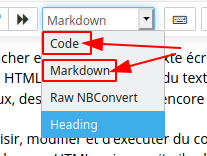
\includegraphics{res/tuto-02.png}

    \hypertarget{arithmuxe9tique}{%
\subsubsection{1.2 --- Arithmétique}\label{arithmuxe9tique}}

    En Python, on peut saisir des combinaires arbitraires d'opérations
arithmétiques, en utilisant notamment les quatre opérations les plus
communes.

        {\scriptsize
    \begin{tcolorbox}[breakable, size=fbox, boxrule=1pt, pad at break*=1mm,colback=cellbackground, colframe=cellborder]
\prompt{In}{incolor}{ }{\boxspacing}
\begin{Verbatim}[commandchars=\\\{\}]
\PY{l+m+mi}{2} \PY{o}{+} \PY{l+m+mi}{5} \PY{o}{*} \PY{p}{(}\PY{l+m+mi}{10} \PY{o}{\PYZhy{}} \PY{l+m+mi}{1} \PY{o}{/} \PY{l+m+mi}{2}\PY{p}{)}
\end{Verbatim}
\end{tcolorbox}
    }

    Quelques remarques

\begin{enumerate}
\def\labelenumi{\arabic{enumi}.}
\tightlist
\item
  Les symboles des quatre opérations sont \texttt{+} (addition),
  \texttt{-} (soustraction), \texttt{*} (multiplication) et \texttt{/}
  (division).
\item
  La priorité des opérations est usuelle et on peut utiliser les
  parenthèses.
\item
  Les espaces sont purement décoratifs : ils rendent plus lisibles mais
  n'agissent pas sur la priorité des opérations
\end{enumerate}

        {\scriptsize
    \begin{tcolorbox}[breakable, size=fbox, boxrule=1pt, pad at break*=1mm,colback=cellbackground, colframe=cellborder]
\prompt{In}{incolor}{ }{\boxspacing}
\begin{Verbatim}[commandchars=\\\{\}]
\PY{l+m+mi}{1}\PY{o}{+}\PY{l+m+mi}{2}     \PY{o}{*} \PY{l+m+mi}{3}
\end{Verbatim}
\end{tcolorbox}
    }

    Remarque bien que l'interprète Python n'accepte pas les expressions qui
sont mal formées ou comportent des erreurs.

    Dans le bloc de code ci-dessous, \textbf{écris} \texttt{1\ +\ *\ 2}.

\textbf{Indique} le type d'erreur affiché.

    Lorsque l'on fait des erreurs de syntaxe car l'expression est mal
formée, l'interprète affiche \texttt{SyntaxError}. Pour aider
l'utilisateur, l'interprète montre l'endroit exact de l'erreur avec le
symbole \texttt{\^{}} qui pointe sous le \texttt{*}.

    \emph{Pour répondre aux questions suivantes, tu peux ajouter des blocs
de texte ou des blocs de code\ldots{}}

En mathématique, est-il possible de \textbf{diviser un nombre par zéro}
?

Et en \textbf{Python} ?

    \hypertarget{les-nombres}{%
\subsubsection{1.3 --- Les nombres}\label{les-nombres}}

    En Python, les nombres sont de deux \emph{types} :

\begin{itemize}
\tightlist
\item
  soit des \textbf{entiers relatifs} (appelés \emph{entiers})
\item
  soit des \textbf{nombres décimaux} (appelés \emph{flottants}).
\end{itemize}

    Attention, les nombres flottans s'écrivent à \emph{l'anglo-saxonne} avec
un point \texttt{.}. Par exemple le nombre \(1,2\) s'écrit en Python
\texttt{1.2}

    \textbf{Indique} ce qu'affiche les commandes suivantes :

\begin{enumerate}
\def\labelenumi{\arabic{enumi}.}
\tightlist
\item
  Commande 1 : \texttt{1,2\ +\ 3,4}.
\item
  Commande 2 : \texttt{1,2\ *\ 3}
\end{enumerate}

\textbf{D'après toi}, à quoi sert le symbole virgule \texttt{,} en
Python ?

    En Python :

\begin{itemize}
\tightlist
\item
  les \emph{entiers} sont de \textbf{taille arbitraire} ;
\item
  les \emph{flottants} en revanche ont une \textbf{capacité limitée} et
  sont souvent des approximations qui ne représentent alors qu'une
  partie des nombres décimaux.
\end{itemize}

Quand tu en as le choix, travaille de préférence avec les entiers.

    \hypertarget{autres-opuxe9rations}{%
\subsubsection{1.4 --- Autres opérations}\label{autres-opuxe9rations}}

    \textbf{Détermine} le type de nombre que l'on obtient lorsque l'on
divise entre eux deux nombres entiers.

    La division avec l'opération \texttt{/} donne un nombre flottant. Ainsi
\texttt{10/2} donne \texttt{5.0} et \texttt{7/2} donne \texttt{3.5}. Ces
deux résultats sont de types \emph{flottant} car ils sont écrits avec
une virgule.

    \textbf{Effectue} \emph{à la main} les divisions euclidiennes :

\begin{itemize}
\tightlist
\item
  \(\frac 72\)
\item
  \(\frac {98}{10}\)
\end{itemize}

    \(7/2\) donne \(3\) et il reste \(1\). L'égalité \(7 = 3 \times 2 + 1\)
est vérifiée.

\(98 / 10\) donne \(9\) et il reste \(8\). L'égalité
\(98 = 9 \times 10 + 8\) est vérifiée.

    Pour effectuer la \textbf{division entière}, il faut utiliser
l'opération \texttt{//}.

\texttt{a\ //\ b} peut être vu comme le plus grand nombre entier
inférieur ou égal à \(a/b\).

Pour obtenir le \textbf{reste de la division euclidienne}, on utilise
l'opération \texttt{\%} (qui se dit \emph{``modulo''}).

    \textbf{Vérifie} à l'aide des opérations \emph{division entière} et
\emph{modulo} les résultats de l'activité précédente.

        {\scriptsize
    \begin{tcolorbox}[breakable, size=fbox, boxrule=1pt, pad at break*=1mm,colback=cellbackground, colframe=cellborder]
\prompt{In}{incolor}{ }{\boxspacing}
\begin{Verbatim}[commandchars=\\\{\}]
\PY{l+m+mi}{7}\PY{o}{/}\PY{o}{/}\PY{l+m+mi}{2}
\end{Verbatim}
\end{tcolorbox}
    }

        {\scriptsize
    \begin{tcolorbox}[breakable, size=fbox, boxrule=1pt, pad at break*=1mm,colback=cellbackground, colframe=cellborder]
\prompt{In}{incolor}{ }{\boxspacing}
\begin{Verbatim}[commandchars=\\\{\}]
\PY{l+m+mi}{7}\PY{o}{\PYZpc{}}\PY{k}{2}
\end{Verbatim}
\end{tcolorbox}
    }

        {\scriptsize
    \begin{tcolorbox}[breakable, size=fbox, boxrule=1pt, pad at break*=1mm,colback=cellbackground, colframe=cellborder]
\prompt{In}{incolor}{ }{\boxspacing}
\begin{Verbatim}[commandchars=\\\{\}]
\PY{l+m+mi}{98} \PY{o}{/}\PY{o}{/} \PY{l+m+mi}{10}
\end{Verbatim}
\end{tcolorbox}
    }

        {\scriptsize
    \begin{tcolorbox}[breakable, size=fbox, boxrule=1pt, pad at break*=1mm,colback=cellbackground, colframe=cellborder]
\prompt{In}{incolor}{ }{\boxspacing}
\begin{Verbatim}[commandchars=\\\{\}]
\PY{l+m+mi}{98} \PY{o}{\PYZpc{}} \PY{l+m+mi}{10}
\end{Verbatim}
\end{tcolorbox}
    }

    L'opération \texttt{**} calcule la \emph{puissance} d'un nombre.

Ainsi, \(10^{3}\) s'écrit \texttt{10\ **\ 3}.

    \textbf{Calculer} dans un bloc de code \(2 ^{1024}\).

Dans un autre bloc de code, \textbf{calculer} \(2,0 ^ {1024}\).

\textbf{Propose} une explication à tes observations.

        {\scriptsize
    \begin{tcolorbox}[breakable, size=fbox, boxrule=1pt, pad at break*=1mm,colback=cellbackground, colframe=cellborder]
\prompt{In}{incolor}{ }{\boxspacing}
\begin{Verbatim}[commandchars=\\\{\}]
\PY{l+m+mi}{2}\PY{o}{*}\PY{o}{*}\PY{l+m+mi}{1024}
\end{Verbatim}
\end{tcolorbox}
    }

        {\scriptsize
    \begin{tcolorbox}[breakable, size=fbox, boxrule=1pt, pad at break*=1mm,colback=cellbackground, colframe=cellborder]
\prompt{In}{incolor}{ }{\boxspacing}
\begin{Verbatim}[commandchars=\\\{\}]
\PY{l+m+mf}{2.0}\PY{o}{*}\PY{o}{*}\PY{l+m+mi}{1024}
\end{Verbatim}
\end{tcolorbox}
    }

    \hypertarget{variables}{%
\subsubsection{1.3 --- Variables}\label{variables}}

    Les résultats calculés peuvent être \textbf{mémorisés} afin d'être
utilisés plus tard.

        {\scriptsize
    \begin{tcolorbox}[breakable, size=fbox, boxrule=1pt, pad at break*=1mm,colback=cellbackground, colframe=cellborder]
\prompt{In}{incolor}{ }{\boxspacing}
\begin{Verbatim}[commandchars=\\\{\}]
\PY{n}{a} \PY{o}{=} \PY{l+m+mi}{1} \PY{o}{+} \PY{l+m+mi}{1}
\end{Verbatim}
\end{tcolorbox}
    }

    La notation \texttt{a\ =} permet de donner un nom à l'information
mémorisée. Ici, l'interprète Python calcule le résultat de
\texttt{1\ +\ 1} et le mémorise dans la \textbf{variable} \texttt{a}.

Aucun résultat n'est affiché. On accède à la valeur mémorisée en
utilisant le nom \texttt{a}.

        {\scriptsize
    \begin{tcolorbox}[breakable, size=fbox, boxrule=1pt, pad at break*=1mm,colback=cellbackground, colframe=cellborder]
\prompt{In}{incolor}{ }{\boxspacing}
\begin{Verbatim}[commandchars=\\\{\}]
\PY{n}{a}
\end{Verbatim}
\end{tcolorbox}
    }

    Affiche maintenant le résultat du calcul \texttt{a\ *\ (a\ +\ 1)}.

        {\scriptsize
    \begin{tcolorbox}[breakable, size=fbox, boxrule=1pt, pad at break*=1mm,colback=cellbackground, colframe=cellborder]
\prompt{In}{incolor}{ }{\boxspacing}
\begin{Verbatim}[commandchars=\\\{\}]
\PY{n}{a} \PY{o}{*} \PY{p}{(}\PY{n}{a}\PY{o}{+}\PY{l+m+mi}{1}\PY{p}{)}
\end{Verbatim}
\end{tcolorbox}
    }

    Le symbole \texttt{=} utilisé pour définir la variable \texttt{a}
désigne une opération d'\textbf{affectation}.

Ce symbole attend à \emph{gauche} un nom de variable et à \emph{droite}
une expression.

On peut donner une nouvelle valeur à la variable \texttt{a} avec une
nouvelle affectation. Cette valeur \emph{remplace} la précédente.

        {\scriptsize
    \begin{tcolorbox}[breakable, size=fbox, boxrule=1pt, pad at break*=1mm,colback=cellbackground, colframe=cellborder]
\prompt{In}{incolor}{ }{\boxspacing}
\begin{Verbatim}[commandchars=\\\{\}]
\PY{n}{a} \PY{o}{=} \PY{l+m+mi}{3}
\PY{n}{a} \PY{o}{*} \PY{p}{(}\PY{n}{a}\PY{o}{+}\PY{l+m+mi}{1}\PY{p}{)}
\end{Verbatim}
\end{tcolorbox}
    }

    Le calcul de la nouvelle valeur de \texttt{a} peut utiliser la valeur
courante de \texttt{a}.

        {\scriptsize
    \begin{tcolorbox}[breakable, size=fbox, boxrule=1pt, pad at break*=1mm,colback=cellbackground, colframe=cellborder]
\prompt{In}{incolor}{ }{\boxspacing}
\begin{Verbatim}[commandchars=\\\{\}]
\PY{n}{a} \PY{o}{=} \PY{n}{a} \PY{o}{+} \PY{l+m+mi}{1}
\PY{n}{a}
\end{Verbatim}
\end{tcolorbox}
    }

    Un nom de variable peut être formé de plusieurs caractères (lettre,
chiffres et tiret bas). Il est recommandé de :

\begin{itemize}
\tightlist
\item
  ne pas utilisé de caractères accentués
\item
  se limiter aux caractères minuscules.
\end{itemize}

        {\scriptsize
    \begin{tcolorbox}[breakable, size=fbox, boxrule=1pt, pad at break*=1mm,colback=cellbackground, colframe=cellborder]
\prompt{In}{incolor}{ }{\boxspacing}
\begin{Verbatim}[commandchars=\\\{\}]
\PY{n}{cube} \PY{o}{=} \PY{n}{a} \PY{o}{*} \PY{n}{a} \PY{o}{*} \PY{n}{a}
\PY{n}{ma\PYZus{}variable} \PY{o}{=} \PY{l+m+mi}{42}
\PY{n}{ma\PYZus{}variable2} \PY{o}{=} \PY{l+m+mi}{2021}
\end{Verbatim}
\end{tcolorbox}
    }

    Une variable peut être imaginée comme un \textbf{emplacement en mémoire}
portant une \textbf{étiquette} et contenant une \textbf{valeur}.

Ainsi, on peut représenter la variable déclarée par \texttt{x\ =\ 1}
comme un emplacement appelé \texttt{x} et contenant la valeur \texttt{1}
par : \(\overset{\texttt{x}}{\fbox{\texttt{1}}}\)

    \hypertarget{uxe9tat}{%
\subsubsection{1.4 --- État}\label{uxe9tat}}

    L'ensemble des associations entre des noms de variables et des valeurs
constitue \textbf{l'état} de l'interprète Python.

Cet état évolue en fonction des instructions exécutées. Les instructions
qui modifient l'état sont dites \emph{à effet de bord}.

    À partir de l'état
\(\overset{\texttt{a}}{\fbox{\texttt{1}}}\overset{\texttt{b}}{\fbox{\texttt{2}}}\overset{\texttt{c}}{\fbox{\texttt{3}}}\overset{\texttt{d}}{\fbox{\texttt{-12}}}\),
les instructions suivantes sont exécutées :

\begin{Shaded}
\begin{Highlighting}[]
\NormalTok{a }\OperatorTok{=}\NormalTok{ c }\OperatorTok{{-}}\NormalTok{ a}
\NormalTok{e }\OperatorTok{=}\NormalTok{ b }\OperatorTok{+}\NormalTok{ c}
\NormalTok{d }\OperatorTok{=}\NormalTok{ a}
\NormalTok{a }\OperatorTok{=} \DecValTok{7}
\end{Highlighting}
\end{Shaded}

\begin{enumerate}
\def\labelenumi{\arabic{enumi}.}
\tightlist
\item
  l'instruction \texttt{a\ =\ c\ -\ a} est interprétée. \textbf{Écrire}
  le nouvel état de l'interprète.
\item
  Ensuite, l'instruction \texttt{e\ =\ b\ +\ c} est interprétée.
  \textbf{Écrire} le nouvel état de l'interprète après cette exécution.
\end{enumerate}

    Cette instruction modifie la valeur de \texttt{a} en fonction des
valeurs de \texttt{c} et de \texttt{a}. L'état sera :
\(\overset{\texttt{a}}{\fbox{\texttt{2}}}\overset{\texttt{b}}{\fbox{\texttt{2}}}\overset{\texttt{c}}{\fbox{\texttt{3}}}\overset{\texttt{d}}{\fbox{\texttt{-12}}}\)

    \href{https://pythontutor.com/visualize.html\#code=a\%20\%3D\%201\%0Ab\%20\%3D\%202\%0Ac\%20\%3D\%203\%0Ad\%20\%3D\%20-12\%0A\%0Aa\%20\%3D\%20c\%20-\%20a\%0Ae\%20\%3D\%20b\%20\%2B\%20c\%0A\%0Ad\%20\%3D\%20a\%0Aa\%20\%3D\%207\&cumulative=true\&curInstr=0\&heapPrimitives=true\&mode=display\&origin=opt-frontend.js\&py=3\&rawInputLstJSON=\%5B\%5D\&textReferences=false}{python
tutor}

    \hypertarget{le-mode-programme}{%
\subsection{2 --- Le mode programme}\label{le-mode-programme}}

    \hypertarget{vscodium}{%
\subsubsection{2.1 --- VSCodium}\label{vscodium}}

    \hypertarget{affichage}{%
\subsubsection{2.2 --- Affichage}\label{affichage}}

    \hypertarget{affichage-des-textes}{%
\subsubsection{2.3 --- Affichage des
textes}\label{affichage-des-textes}}

    \hypertarget{suxe9quence-dinstructions}{%
\subsubsection{2.4 --- Séquence
d'instructions}\label{suxe9quence-dinstructions}}

    

    \hypertarget{interagir-avec-lutilisateur}{%
\subsubsection{2.5 --- Interagir avec
l'utilisateur}\label{interagir-avec-lutilisateur}}

    \hypertarget{un-programme-complet}{%
\subsubsection{2.6 --- Un programme
complet}\label{un-programme-complet}}

    \hypertarget{repruxe9sentation-de-lexuxe9cution}{%
\subsubsection{2.7 --- Représentation de
l'exécution}\label{repruxe9sentation-de-lexuxe9cution}}

    \hypertarget{exemple-de-bibliothuxe8que-turtle}{%
\subsection{\texorpdfstring{3 --- Exemple de bibliothèque
\texttt{Turtle}}{3 --- Exemple de bibliothèque Turtle}}\label{exemple-de-bibliothuxe8que-turtle}}

    


    % Add a bibliography block to the postdoc
    
    
    
\end{document}
